\section{Introduction}
Social Networks have created a new realm in the world of Computer Science. Everyone is constantly looking into ways of integrating the knowledge from existing social networks to make their systems more personal for their end users. Microsoft now ranks results, in its BING search, for a user using the search history from his/her social network~\cite{M2011}. There are also works on how probable a user performs an action given his/her friend committed the same action before~\cite{DJE2003}. 

At the other end of the spectrum are the spatial networks. With the ever increasing number of wearables everyday like Jawbone, fitbit, smart watches (pebble, apple watch) there is an abundance of data in this realm too. Importantly with the rapid increase in the number of mobile phone users, this data is already being tied to Social Network data and the two realms are coming together. Popular social network sites like Facebook have a number of features which prompt users to add spatial information like checkins, traveling posts, geotagged photos etc.

And this paper is all about bringing these two even closer. Feeding results from this paper into an existing recommendation systems, we can predict what your best friend would have suggested to you if you wanted to go to an authentic Sushi place in SFO. Imagine restaurant recommendations from Google, are more personalized for a location instead of listing them by average user rating. To answer such queries we need to traverse a social network and filter recommendations which fall in a given location. However we want minimum latency for such queries for the best user experience on a current social network like Facebook which has around 1.59 billion active users monthly~\footnote{\href{http://www.statista.com/statistics/264810/number-of-monthly-active-facebook-users-worldwide/}{Facebook Active Users Stats Link}}. These graphs can be really dense as, each person in the world is connected to every other person by only an average of three and a half other people!~\cite{Taa}. So we need a way to answer shortest path reachability queries with a spatial predicate quickly even in such dense graphs (that is conditioned on a region).

\begin{figure}[t]
	\centering
	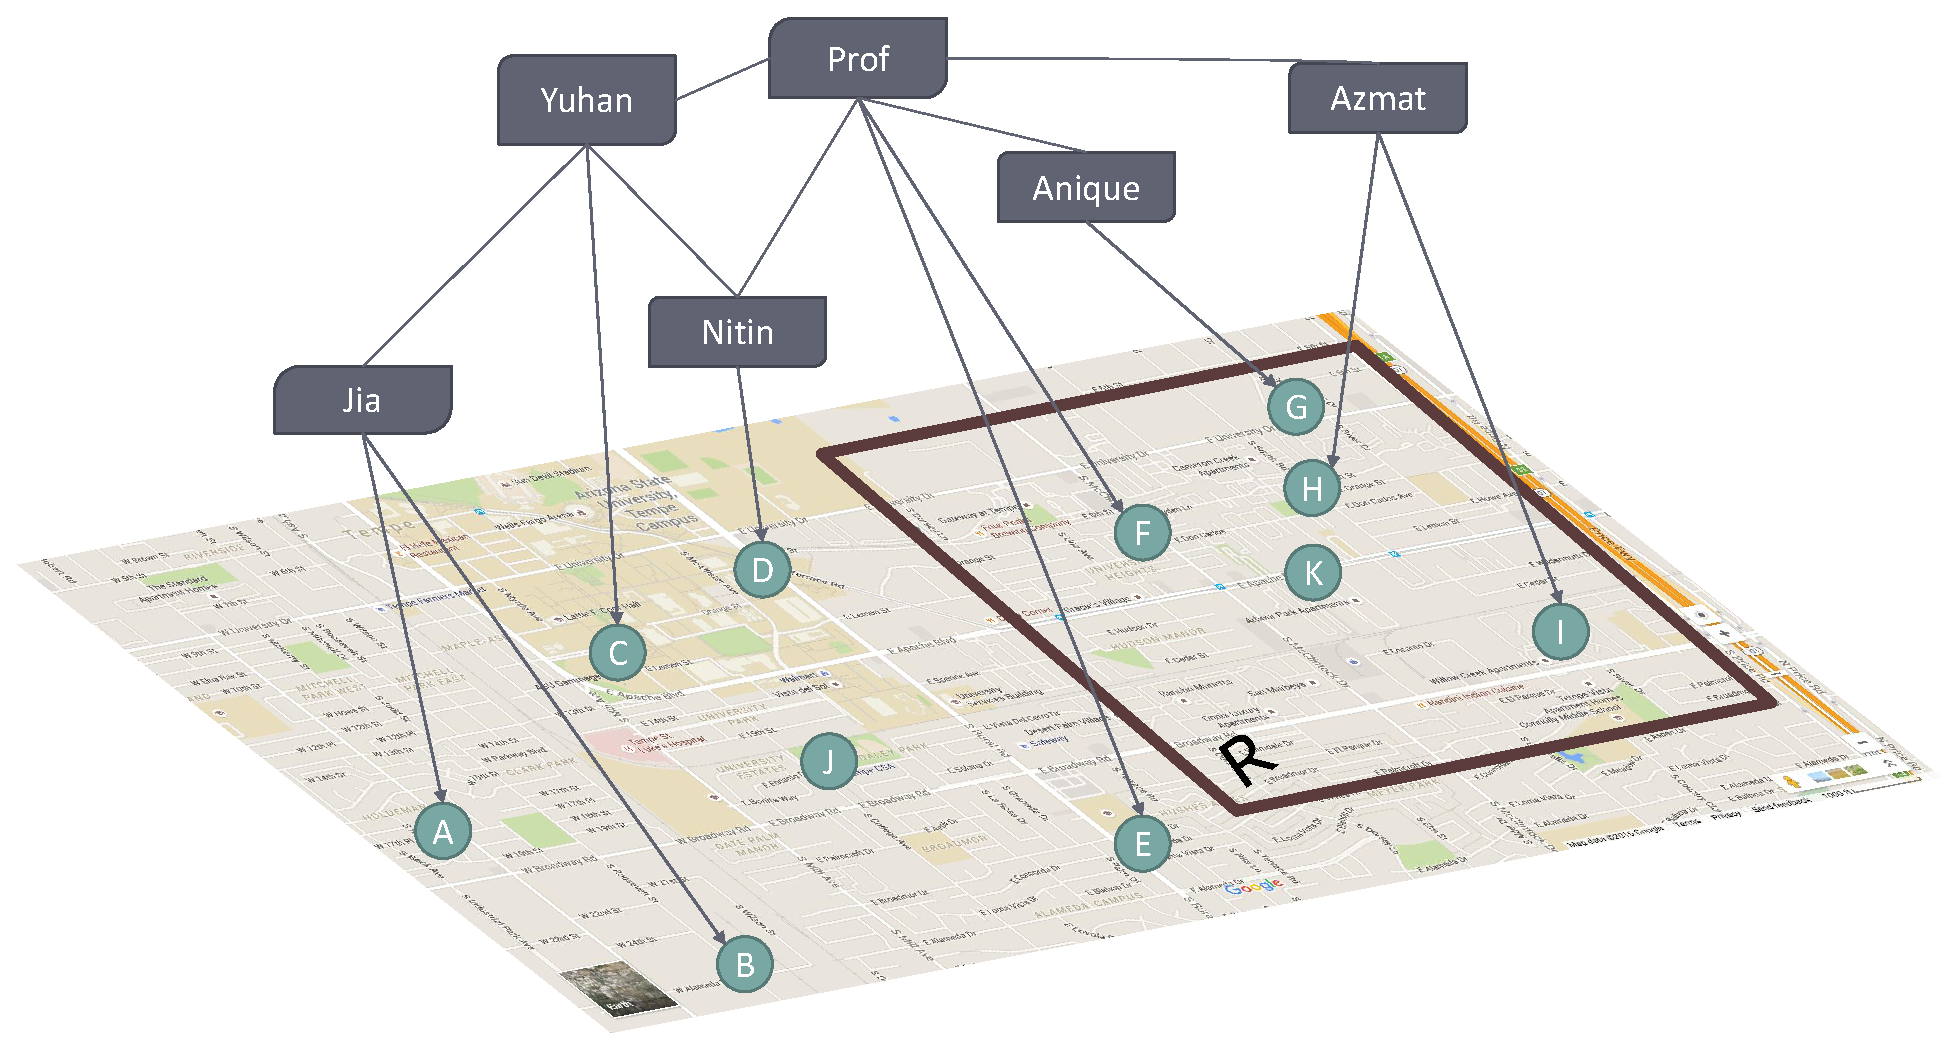
\includegraphics[width=0.88\linewidth]{images/begin_example.eps}
	\caption{A motivation example}
	\label{fig:begin-example}
\end{figure}

Consider a restaurant recommendation system like Yelp. Every registered user can have multiple friends and also check-ins at multiple restaurants using this service. A small example from such a service would look like the one shown in Figure \ref{fig:begin-example} where Jia, Yuhan, Nitin, Prof, Anique, Azamat are people and letters from A to I are restaurants. Restaurants are also marked at the respective locations on a map. Edges between people indicate they are friends like in any social network and edges from a person to a restaurant means he/she checked-in at that location. Assume we want to recommend a restaurant to Jia in the marked region R and that all restaurants have the same average customer rating as 4.0. Any existing system would naturally return restaurants that fall in R in some random order as all of them are equally good. However, we can see Jia is close to Prof than to Anique or Azamat. Recommending restaurant F before G, H and I would make Jia happier as Prof and Jia are more similar in their tastes. Therefore, in order to provide good recommendations, we should consider both the spatial and social proximity in the search.

In this paper we propose a \textit{range reach paths} (RRP) query which finds top-k shortest paths in a graph/network considering both the social and spatial components. Our key contributions are:
\begin{itemize}
	\item We study the socio-spatial graph problem describing the challenge more formally and understand the need to solve this more efficiently.
	\item We propose indices on social and spatial domains of the graph which form the pre-processing stage of the solution. Here we store the data in an organized manner to filter graph based on spatial (region of interest) and social constraints (top-k shortest paths) at query time.
	\item We propose a robust algorithm which uses above indices to answer topk-k socio-spatial query using a modified landmark based A* algorithm by combining it with a spatial search.
	\item We experimentally evaluate the proposed approach with different parameter combinations on Yelp dataset. The experiments shows that our approach can achieve at least 5 times faster than existing approaches. %Experimentally prove our algorithms on real datasets like Yelp to understand internal details about each index and when using one index over the other is more fruitful.
\end{itemize}

% TODO: paper overview.
%We tested our approach on various types of graphs with different parameter combinations only to find that our idea outperforms existing solutions by at least 500\%. Detailed explanations can be found in the experiments section.